% ---
% Arquivo com a metodologia do Trabalho de Conclusão de Curso dos alunos
% Gabriel Takaoka Nishimura, Felippe Demarqui Ramos e Vivian Kimie Isuyama 
% da Escola Politécnica da Universidade de São Paulo
% ---
	\chapter{Metodologia}\label{cap-metodologia}
	
	\section{Hardware}\label{sec-hardware}
	
	Explica as escolhas feitas de hardware.
	
	% ---
	\subsection{FPGA}
	% ---
	
	Explicação do porquê foi escolhido FPGA
	
	\subsubsection{Opções Consideradas}\label{fpga-opcoes}
	
	Explicação de quais foram as opções consideradas.
	
	\subsubsection{Tabela Comparativa}\label{fpga-comparativo}
	
	Tabela de opções consideradas.
	
	% ---
	\subsection{Microcontrolador}
	% ---
	
	Explicação do porquê foi escolhido microcontrolador
	
	\subsubsection{Opções Consideradas}\label{uc-opcoes}
	
	\lipsum[14]
	
	\subsubsection{Tabela Comparativa}\label{uc-comparativo}
	
	\lipsum[15]
	
	% ---
	\subsection{LED}
	% ---
	
	\lipsum[2]
	
	
	% ---
	\subsection{Circuito de Amplificação}
	% ---
	
	Com intuito de reduzir o ruido da luz ambiente, o circuito a seguir (\autoref{fig_opampdif}) foi proposto para o projeto:
	
	\begin{figure}[htb]
		\caption{\label{fig_opampdif}Circuito amplificador de diferenças.}
		\begin{center}
			%  trim={<left> <lower> <right> <upper>} 
			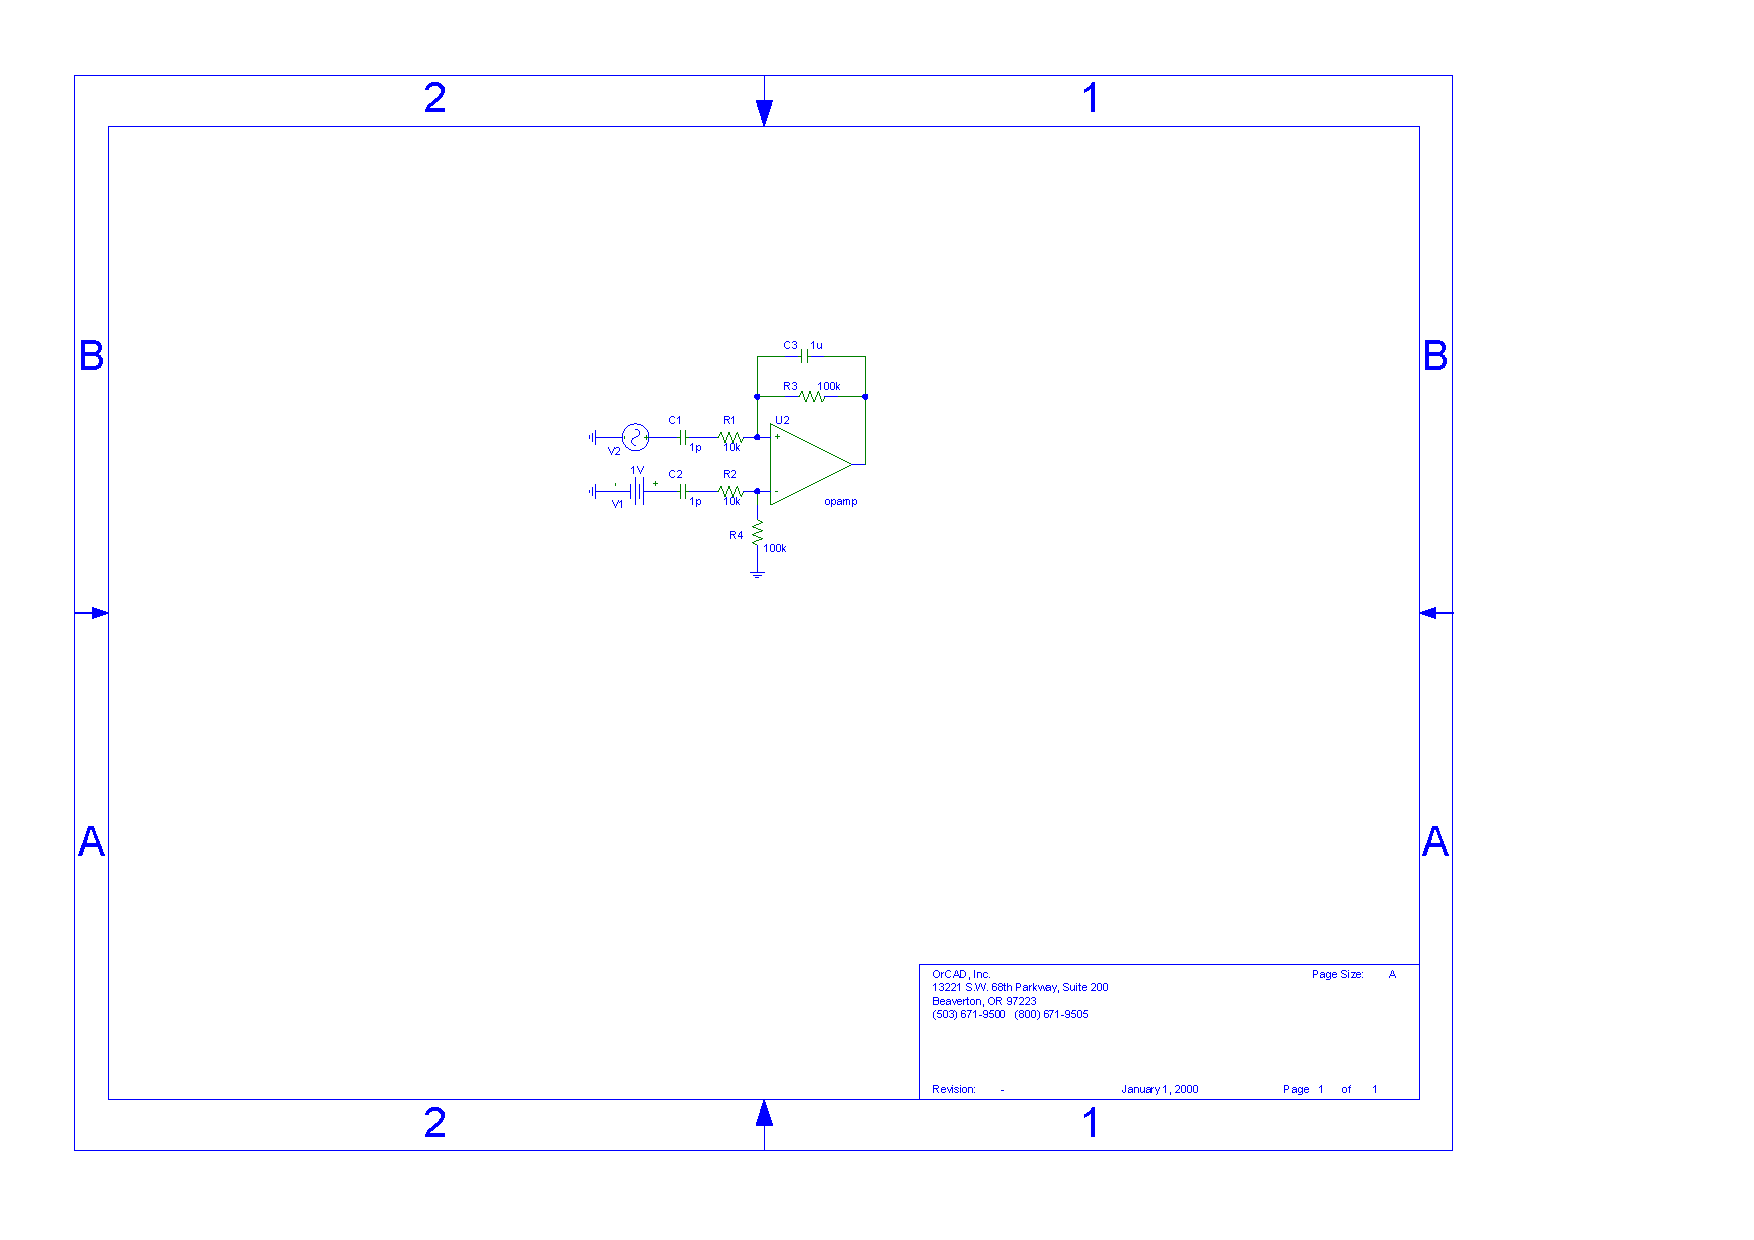
\includegraphics[width=0.5\textwidth, trim={9.5cm 11.2cm 15cm 5.76cm},clip]{opamp-dif.pdf}
		\end{center}
		\legend{Fonte: Próprios autores}
	\end{figure}
	
	Explicação de porque foi escolhido o circuito com ampop em modo diferencial para o projeto.
	
	% ---
	\subsection{LED}
	% ---
	
	Explicação de porque foi escolhido aquele LED para o projeto.
	
	\section{Software}\label{sec-software}
	
	Explica as escolhas feitas no aspecto do software do projeto.
	
	% ---
	\subsection{VHDL}
	% ---
	
	Explicação do porquê foi escolhido VHDL
	
	\subsubsection{Opções Consideradas}\label{vhdl-opcoes}
	
	Explicação de quais foram as opções consideradas.
	
	\subsubsection{Tabela Comparativa}\label{vhdl-comparativo}
	
	Tabela de opções consideradas.
	
	
	% ---
	\subsection{Quartus}
	% ---
	
	Explicação do porquê foi escolhido Quartus
	
	\subsubsection{Opções Consideradas}\label{quartus-opcoes}
	
	\lipsum[10]
	
	\subsubsection{Tabela Comparativa}\label{quartus-comparativo}
	
	\lipsum[11]
	
	% ---
	\subsection{Android}
	% ---
	
	Explicação do porquê foi escolhido Android.
